\begin{appendices}
  
\chapter{APDL-TransForm Language Introduction}
\label{app:tf-getting-started}

TODO

\chapter{APDL Abstract Syntax Tree Implementation}
\label{app:apdl_ast_implementation}

\section*{MainParsers.scala}
\scalafile{../APDL/src/main/scala/apdl/parser/MainParsers.scala}

\section*{DefineParsers.scala}
\scalafile{../APDL/src/main/scala/apdl/parser/DefineParsers.scala}

\section*{TransformDslParser.scala}
\scalafile{../APDL/src/main/scala/apdl/parser/TransformDslParser.scala}

\section*{TransformDslAst.scala}
\scalafile{../APDL/src/main/scala/apdl/parser/TransformDslAst.scala}

\chapter{APDL EBNF Diagrams}
\label{app:apdl_ebnf_diagramm}

\section*{program}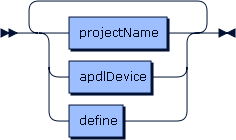
\includegraphics[scale=0.7]{img/ebnf_grammar/program}
\section*{projectName}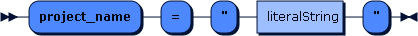
\includegraphics[scale=0.7]{img/ebnf_grammar/projectName}
\section*{apdlDevice}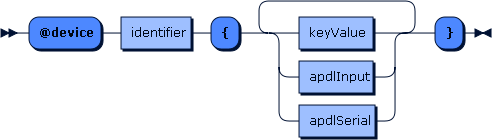
\includegraphics[scale=0.7]{img/ebnf_grammar/apdlDevice}
\section*{defines}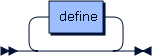
\includegraphics[scale=0.7]{img/ebnf_grammar/defines}
\section*{define}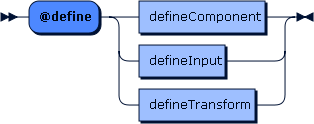
\includegraphics[scale=0.7]{img/ebnf_grammar/define}
\section*{defineComponent}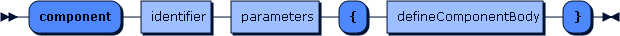
\includegraphics[scale=0.7]{img/ebnf_grammar/defineComponent}

\section*{apdlInput}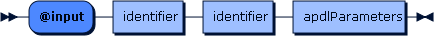
\includegraphics[scale=0.7]{img/ebnf_grammar/apdlInput}
\section*{apdlSerial}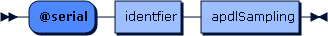
\includegraphics[scale=0.7]{img/ebnf_grammar/apdlSerial}
\section*{apdlParameters}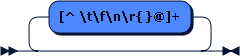
\includegraphics[scale=0.7]{img/ebnf_grammar/apdlParameters}
\section*{apdlSampling}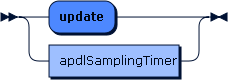
\includegraphics[scale=0.7]{img/ebnf_grammar/apdlSampling}
\section*{apdlSamplingTimer}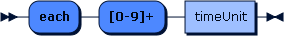
\includegraphics[scale=0.7]{img/ebnf_grammar/apdlSamplingTimer}
\section*{timeUnit}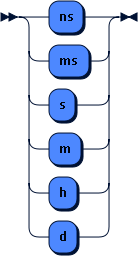
\includegraphics[scale=0.7]{img/ebnf_grammar/timeUnit}
\section*{type}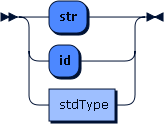
\includegraphics[scale=0.7]{img/ebnf_grammar/type}
\section*{stdType}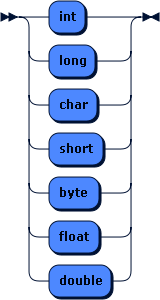
\includegraphics[scale=0.7]{img/ebnf_grammar/stdType}
\section*{arg}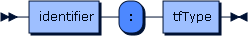
\includegraphics[scale=0.7]{img/ebnf_grammar/arg}

\section*{defineInput}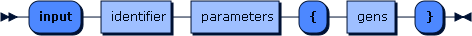
\includegraphics[scale=0.7]{img/ebnf_grammar/defineInput}
\section*{defineTransform}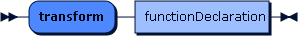
\includegraphics[scale=0.7]{img/ebnf_grammar/defineTransform}
\section*{defineComponentBody}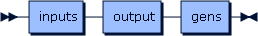
\includegraphics[scale=0.7]{img/ebnf_grammar/defineComponentBody}

\section*{parameters}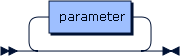
\includegraphics[scale=0.7]{img/ebnf_grammar/parameters}
\section*{parameter}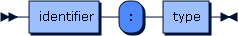
\includegraphics[scale=0.7]{img/ebnf_grammar/parameter}

\section*{inputs}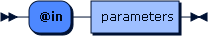
\includegraphics[scale=0.7]{img/ebnf_grammar/inputs}
\section*{output}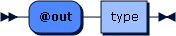
\includegraphics[scale=0.7]{img/ebnf_grammar/output}
\section*{gens}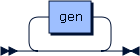
\includegraphics[scale=0.7]{img/ebnf_grammar/gens}
\section*{gen}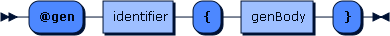
\includegraphics[scale=0.7]{img/ebnf_grammar/gen}
\section*{genBody}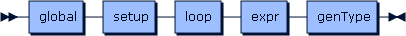
\includegraphics[scale=0.7]{img/ebnf_grammar/genBody}
\section*{global}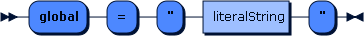
\includegraphics[scale=0.7]{img/ebnf_grammar/global}
\section*{setup}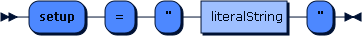
\includegraphics[scale=0.7]{img/ebnf_grammar/setup}
\section*{loop}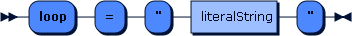
\includegraphics[scale=0.7]{img/ebnf_grammar/loop}
\section*{expr}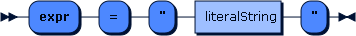
\includegraphics[scale=0.7]{img/ebnf_grammar/expr}
\section*{genType}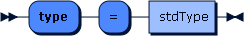
\includegraphics[scale=0.7]{img/ebnf_grammar/genType}
\section*{literalString}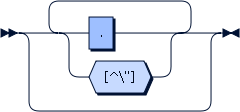
\includegraphics[scale=0.7]{img/ebnf_grammar/literalString}

\section*{returnType}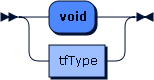
\includegraphics[scale=0.7]{img/ebnf_grammar/returnType}
\section*{tfType}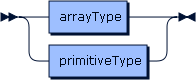
\includegraphics[scale=0.7]{img/ebnf_grammar/tfType}
\section*{primitiveType}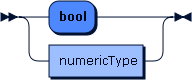
\includegraphics[scale=0.7]{img/ebnf_grammar/primitiveType}
\section*{numericType}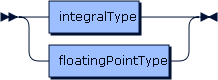
\includegraphics[scale=0.7]{img/ebnf_grammar/numericType}
\section*{arrayType}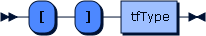
\includegraphics[scale=0.7]{img/ebnf_grammar/arrayType}
\section*{integralType}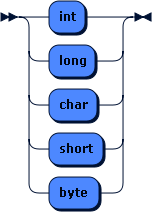
\includegraphics[scale=0.7]{img/ebnf_grammar/integralType}
\section*{floatingPointType}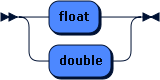
\includegraphics[scale=0.7]{img/ebnf_grammar/floatingPointType}

\section*{constantExpr}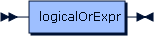
\includegraphics[scale=0.7]{img/ebnf_grammar/constantExpr}
\section*{logicalOrExpr}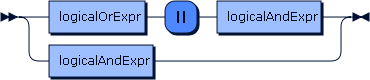
\includegraphics[scale=0.7]{img/ebnf_grammar/logicalOrExpr}
\section*{logicalAndExpr}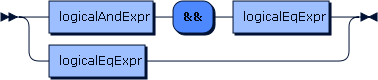
\includegraphics[scale=0.7]{img/ebnf_grammar/logicalAndExpr}
\section*{logicalEqExpr}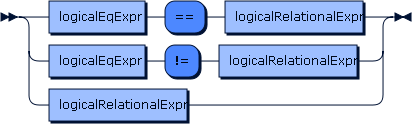
\includegraphics[scale=0.7]{img/ebnf_grammar/logicalEqExpr}
\section*{logicalRelationalExpr}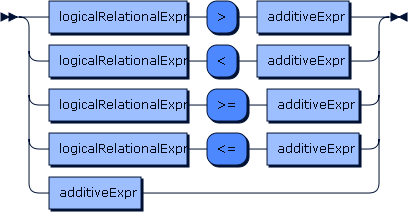
\includegraphics[scale=0.7]{img/ebnf_grammar/logicalRelationalExpr}
\section*{additiveExpr}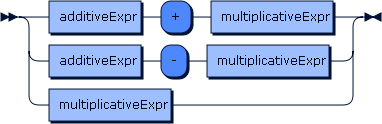
\includegraphics[scale=0.7]{img/ebnf_grammar/additiveExpr}
\section*{multiplicativeExpr}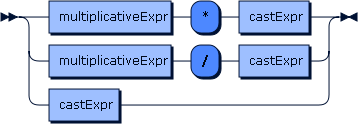
\includegraphics[scale=0.7]{img/ebnf_grammar/multiplicativeExpr}
\section*{castExpr}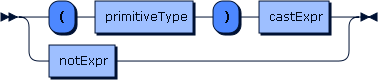
\includegraphics[scale=0.7]{img/ebnf_grammar/castExpr}
\section*{notExpr}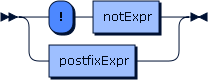
\includegraphics[scale=0.7]{img/ebnf_grammar/notExpr}
\section*{postfixExpr}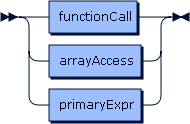
\includegraphics[scale=0.7]{img/ebnf_grammar/postfixExpr}
\section*{primaryExpr}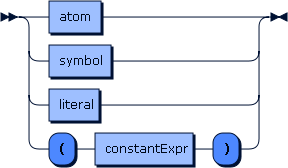
\includegraphics[scale=0.7]{img/ebnf_grammar/primaryExpr}
\section*{functionCall}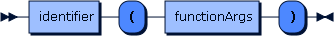
\includegraphics[scale=0.7]{img/ebnf_grammar/functionCall}
\section*{functionArgs}\includegraphics[scale=0.7]{img/ebnf_grammar/functionArgs}
\section*{arrayAccess}\includegraphics[scale=0.7]{img/ebnf_grammar/arrayAccess}
\section*{atom}\includegraphics[scale=0.7]{img/ebnf_grammar/atom}
\section*{symbol}\includegraphics[scale=0.7]{img/ebnf_grammar/symbol}
\section*{literal}\includegraphics[scale=0.7]{img/ebnf_grammar/literal}
\section*{assignExpr}\includegraphics[scale=0.7]{img/ebnf_grammar/assignExpr}
\section*{identifier}\includegraphics[scale=0.7]{img/ebnf_grammar/identifier}

\section*{functionDeclaration}\includegraphics[scale=0.7]{img/ebnf_grammar/functionDeclaration}
\section*{functionHeader}\includegraphics[scale=0.7]{img/ebnf_grammar/functionHeader}
\section*{functionBody}\includegraphics[scale=0.7]{img/ebnf_grammar/functionBody}
\section*{block}\includegraphics[scale=0.7]{img/ebnf_grammar/block}
\section*{statement}\includegraphics[scale=0.7]{img/ebnf_grammar/statement}
\section*{selectionStatement}\includegraphics[scale=0.7]{img/ebnf_grammar/selectionStatement}
\section*{loops}\includegraphics[scale=0.7]{img/ebnf_grammar/loops}
\section*{jump}\includegraphics[scale=0.7]{img/ebnf_grammar/jump}
\section*{exprStatement}\includegraphics[scale=0.7]{img/ebnf_grammar/exprStatement}

\section*{ifThenElse}\includegraphics[scale=0.7]{img/ebnf_grammar/ifThenElse}
\section*{ifThen}\includegraphics[scale=0.7]{img/ebnf_grammar/ifThen}
\section*{while}\includegraphics[scale=0.7]{img/ebnf_grammar/while}
\section*{doWhile}\includegraphics[scale=0.7]{img/ebnf_grammar/doWhile}

\section*{declaration}\includegraphics[scale=0.7]{img/ebnf_grammar/declaration}
\section*{newArray}\includegraphics[scale=0.7]{img/ebnf_grammar/newArray}
\section*{arrayInit}\includegraphics[scale=0.7]{img/ebnf_grammar/arrayInit}
\section*{newVal}\includegraphics[scale=0.7]{img/ebnf_grammar/newVal}
\section*{newVar}\includegraphics[scale=0.7]{img/ebnf_grammar/newVar}


\chapter{APDL Recursive Inclusion Algorithm Implementation in Scala}
\label{app:algo_recursive_construct}

\begin{scalacode}
def generateInputs(out: ApdlPrintWriter): Unit = {
  // Generate default input
  debug(s"\tGenerate default inputs")
  generateDefaultInputs(out)
  // Make the symbolTable for non-default input
  debug(s"\tGenerate non default inputs")
  generateNonDefaultInputs(out)
}

def generateNonDefaultInputs(out: ApdlPrintWriter): Unit = {
  val inputs = device.inputs
  val nonDefaultInputs = inputs.filter(isNonDefault)

  // For each inputs, take the ones who are generable
  def process(inputs: List[ApdlInput]): Unit = if (inputs.nonEmpty) {
    val (generableInputs, nonGenerableInputs) = inputs.partition(isGenerable)
    generableInputs.foreach { i =>
      if (isTransform(i)) {
        val sourceInput = symbolTable.get(i.args.head) match {
          case default: InputDefault => default
          case transformed: InputTransformed => transformed
          case componented: InputComponented => componented
          case _ => throw new ApdlProjectException(s"Can't find source input for input ${i.identifier}")
        }
        val definition = defines.find(_.identifier == i.defineInputIdentifier) match {
          case Some(value) => value
          case None => throw new ApdlProjectException(s"Unknow define for input ${i.identifier}")
        }
        assume(definition.isInstanceOf[ApdlDefineTransform])

        // code generation
        val functionDecl = definition.asInstanceOf[ApdlDefineTransform].functionDecl

        if (!symbolTable.contains(functionDecl.header.identifier)) {
          // A transform is a function
          out.printlnFunction {
            s"""
                | // Transform ${functionDecl.header.identifier}
                | ${transformCodeGen(functionDecl)}
                | // End transform ${functionDecl.header.identifier}
            """.stripMargin
          }
          // Add the transform into the symbol table
          symbolTable.add(functionDecl.header.identifier, Transform(functionDecl))
        }
        symbolTable.add(i.identifier, InputTransformed(i.identifier, definition.asInstanceOf[ApdlDefineTransform], sourceInput))

      } else if (isComponented(i)) {

        val definition = defines.find(_.identifier == i.defineInputIdentifier) match {
          case Some(value) => value
          case None => throw new ApdlProjectException(s"Unknow define for input ${i.identifier}")
        }

        assume(definition.isInstanceOf[ApdlDefineComponent])

        val component = definition.asInstanceOf[ApdlDefineComponent]

        val nbNonInputs = component.parameters.length
        val args = i.args.drop(nbNonInputs)
        val sourceInputs: List[Input] = symbolTable.gets(args).map {
          case default: InputDefault => default
          case transformed: InputTransformed => transformed
          case componented: InputComponented => componented
          case _ => throw new ApdlProjectException(s"Can't find source input for input ${i.identifier}")
        }


        symbolTable.add(i.identifier, InputComponented(i.identifier, definition.asInstanceOf[ApdlDefineComponent], sourceInputs))

      } else {
        // something is wrong...
        throw new ApdlProjectException(s"Input ${i.identifier} from device ${device.name} encountered some problems")
      }
    }
    process(nonGenerableInputs)
  }

  process(nonDefaultInputs)
}

def isTransform(input: ApdlInput): Boolean = defines.find {
  case ApdlDefineTransform(functionDecl) => functionDecl.header.identifier == input.defineInputIdentifier
  case _ => false
} match {
  case Some(value) =>
    assert(value.isInstanceOf[ApdlDefineTransform])
    assert(input.args.length == 1)
    true
  case None => false
}

def isComponented(input: ApdlInput): Boolean = defines.find {
  case component: ApdlDefineComponent => component.identifier == input.defineInputIdentifier
  case _ => false
} match {
  case Some(value) =>
    assert(value.isInstanceOf[ApdlDefineComponent])
    true
  case None => false
}

def isGenerable(input: ApdlInput): Boolean = {
  if (isTransform(input)) {
    assert(input.args.length == 1)
    val sourceInput = input.args.head
    symbolTable.contains(sourceInput)
  }
  else if (isComponented(input)) {
    val componentDefine = defines.find(_.identifier == input.defineInputIdentifier) match {
      case Some(value) => value match {
        case component: ApdlDefineComponent => component
        case _ => throw new ApdlProjectException(s"Unexpected definition found for input ${input.identifier} from device ${device.name}")
      }
      case None => throw new ApdlProjectException(s"Unknow define component for input ${input.identifier} from device ${device.name}")
    }
    val nbNonInputs = componentDefine.parameters.length
    val args = input.args.drop(nbNonInputs)
    args.forall(symbolTable.contains)
  }
  else {
    throw new ApdlProjectException(s"Wrong input type for input ${input.identifier} from device ${device.name}")
  }
}

def isNonDefault(input: ApdlInput): Boolean = {
  !isDefault(input)
}

def isDefault(input: ApdlInput): Boolean = {
  defines.find(_.identifier == input.defineInputIdentifier) match {
    case Some(definition) => definition match {
      case _: ApdlDefineInput => true
      case _: ApdlDefineComponent => false
      case _: ApdlDefineTransform => false
    }
    case None =>
      throw new ApdlProjectException(s"Unknow type for input ${input.identifier}")
  }
}

// Generate the default input inside the symbol table
def generateDefaultInputs(out: ApdlPrintWriter): Unit = device.inputs.foreach { input =>
  defines.find(_.identifier == input.defineInputIdentifier) match {
    case Some(definition) => definition match {
      case ApdlDefineInput(name, parameters, gens) =>
        // A default input

        val gen = gens.getOrElse(framework.identifier, throw new ApdlProjectException(s"Unknow framework $framework for input definition : $name"))

        implicit val args = zipArgWithIdentifier(input.args, parameters, List()) + ("id" -> IdGenerator.nextVariable(input.identifier))

        out.printlnGlobal(gen.global.replaceWithArgs)
        out.printlnSetup(gen.setup.replaceWithArgs)
        out.printlnLoop(gen.loop.replaceWithArgs)

        symbolTable.add(input.identifier, InputDefault(
          input.identifier,
          definition.asInstanceOf[ApdlDefineInput],
          input.args,
          gen.expr.replaceWithArgs))
      case _ =>
    }
    case None => throw new ApdlProjectException(s"Unknow type for input ${input.identifier}")
  }
}
\end{scalacode}

\chapter{Generators Implementation for Property-based Testing}
\label{app:generators_property_based_testing}

\section*{GeneratorUtils.scala}
\scalafile{../APDL/src/test/scala/GeneratorUtils.scala}

\chapter{APDL Code Generator for Property-based Testing}
\label{app:apdl_code_generator_for_test}

\section*{DslApdlBackendGenerators.scala}
\scalafile{../APDL/src/main/scala/apdl/parser/DslApdlBackendGenerators.scala}

\section*{TransformApdlBackendGenerators.scala}
\scalafile{../APDL/src/main/scala/apdl/parser/TransformApdlBackendGenerators.scala}

\chapter{Implementation of the Preprocessor's Tests}
\label{app:includes_tests}

\section*{IncludeTest.scala}
\scalafile{../APDL/src/test/scala/IncludeTest.scala}

\chapter{APDL Component file}
\label{app:apdl_component_apdl}

\section*{apdl\_component.apdl}
\begin{apdlcode}
@define input analogInput pin:str {
    @gen mbed {
        global = "AnalogIn @id(@pin);"
        setup = ""
        loop = ""
        expr = "@id.read()"
        type = float
    }
    @gen arduino {
        global = ""
        setup = ""
        loop = ""
        expr = "analogRead(@pin)"
        type = int
    }
}

@define input digitalInput pin:str {
    @gen mbed {
        global = "DigitalIn @id(Dpin);"
        setup = ""
        loop = ""
        expr = "@id.read()"
        type = float
    }
    @gen arduino {
        global = ""
        setup = ""
        loop = ""
        expr = "digitalRead(@pin)"
        type = int
    }
}
\end{apdlcode}

\end{appendices}
